\documentclass{article}
\usepackage{graphicx}
\usepackage{amsmath}
\usepackage{pgfplots}
\usepackage{physics}
\usepackage{cancel}
\usepackage{enumitem}
\usepackage{txfonts}

\pgfplotsset{compat=1.18}

\usepackage[a4paper, top=1cm, bottom=2cm, left=2cm, right=2cm, includehead, includefoot]{geometry}

\begin{document}

\noindent
Physics 4A - Classical Mechanics \hfill Prof. Roger King

\noindent\rule{\textwidth}{0.4pt}

\begin{center}
    \textbf{\LARGE Homework 5} \\
    \vspace{12pt}
    \large Aaron W. Tarajos \\
    \textit{\today}
\end{center}

\noindent\rule{\textwidth}{0.4pt}

\section*{Problem 1}
A ball thrown at 20.0 m/s at angle $\theta$ below the horizontal from a cliff of height $H$ lands 69.0 m from the base 4.00 s later. Find $\theta$ and $H$.

\subsection*{Solution}
We can solve for $\theta$ using
\begin{align*}
	\Delta x &= \left(v_0\cos\theta\right)t \\
	\frac{\Delta x}{v_0 t} &= \cos\theta \\
	\theta &= \arccos\left(\frac{\Delta x}{v_0 t}\right)
\end{align*}
and because the angle is negative we have
\[
	\theta = -\left( \arccos\left(\frac{69.0}{20.0 \cdot 4.00} \right)\right) = \boxed{-30.402^\circ}
\]
Then using

\begin{equation}
	\Delta y = x \tan\theta - \frac{gx^2}{2\left(v_0 \cos\theta\right)^2}
\end{equation}
we find that the height of the cliff is
\[
	\Delta y = 69 \tan\left( -30.402 \right) - \frac{9.81 \left( 69.0 \right)^2 }{2 \left(20 \cos\left( -30.402 \right) \right)^2 } = \boxed{118.966\ \text{m}}
\]

\section*{Problem 2}
A ball is thrown at 14.0 m/s at 45$^\circ$ above the horizontal. Someone located 30.0 m away along line of the path starts to run just as the ball is thrown. How fast, and in which direction, must the person run to catch the ball at the level from which it was thrown?

\subsection*{Solution}
The range of the ball is given by

\begin{equation}
	R = \frac{v_0^2}{g}\sin2\theta
\end{equation}
We find the time they need to be there by
\begin{equation}
	t = \frac{R}{v_0 \cos\theta}
\end{equation}
If the catcher is at some position $p$, their velocity (direction and speed) to get to location $R$ at time $t$ is given by
\begin{equation}
	v = \frac{R-p}{t}
\end{equation}
\begin{align*}
	v &= \left(\frac{14.0^2}{9.81}\sin(90) - 30\right) \cdot \left(\frac{14.0 \cos(45)}{\frac{14.0^2}{9.81}\sin(90)}\right) \\
	  &= \boxed{-4.965\ \text{m/s}}
\end{align*}

\section*{Problem 3}
If a baseball player can throw a ball at 45$^\circ$ to a point 100 m away horizontally to the initial
vertical level, how high could he throw it vertically upward?

\subsection*{Solution}
We solve for initial velocity using
\begin{align*}
	R &= \frac{v_0^2}{g}\sin 2\theta \\
	v_0 &= \sqrt{\frac{Rg}{\sin 2\theta}}
\end{align*}
and then the maximum height of ball thrown vertically at this velocity is given by
\begin{align*}
	v^2 &= v_0^2  + 2a\Delta y \\
	\Delta y &= \frac{v^2-v_0^2}{2a}
\end{align*}
The final velocity is zero so we have

\[
	\Delta y = \frac{-\left( \frac{Rg}{\sin 2\theta} \right)}{(2)(a)} = \frac{-\left( \frac{100 \cdot 9.81}{\sin(90)} \right)}{(2)(-9.81)} = \boxed{50\ \text{m}}
\]

\section*{Problem 4}
A motorcyclist plans to jump across a gorge width 32.0 m. He takes off on an 18.0$^\circ$ ramp.
What minimum speed does he require if he lands at the initial level?

\subsection*{Solution}
We can use the velocity equation from Problem 3 to solve for the minimum speed
\[
	v_0 = \sqrt{\frac{Rg}{\sin 2\theta}} = \sqrt{\frac{32\cdot 9.81}{\sin 2(18)}} = \boxed{23.110\ \text{m/s}}
\]

\section*{Problem 5}
A projectile fired from the ground has a velocity $\vec{v} = 24.0 \hat i - 8.00 \hat j$ m/s at a height of
9.10 m. Find: (a) the initial velocity; (b) the maximum height

\subsection*{Solution}
\subsubsection*{Part a:}
The horizontal initial velocity is constant and given a $24.0 \hat i$ and we can solve for vertical initial velocity using
\begin{align*}
	v_{0y} &= \sqrt{v_y^2 - 2a \Delta y} \\
	       &= \sqrt{8.0^2 - 2(-9.81)(9.10)} \\
	       &= 15.574 \hat j\ \text{m/s}
\end{align*}
So the initial velocity is

\[
	\boxed{v_{0y} = 24.0 \hat i + 15.574 \hat j\ \text{m/s}}
\]

\subsubsection*{Part b:}
The maximum height occurs at $v_{0y} = 0$ using
\begin{equation}
	\Delta y = \frac{v_y^2 - v_{0y}^2}{2a}
\end{equation}
we find that the maximum height is
\begin{align*}
	\Delta y &= \frac{0.0^2 - \sqrt{8.0^2 - 2(-9.81)(9.10)}}{2(-9.81)}^2 \\
		 &= \frac{0.0^2 - \left(8.0^2 - 2(-9.81)(9.10)\right)}{2(-9.81)} \\
		 &= \boxed{12.362\ \text{m}}
\end{align*}

\section*{Problem 6}
The figure below shows a conical pendulum. It consists of a bob is suspended at the end of a
string and describes a horizontal circle at a constant speed of 1.28 m/s. If the length of the
string is 1.20 m and it makes an angle of 20$^\circ$ with the vertical, find the acceleration of the bob.

\begin{figure}[ht]
    \centering
    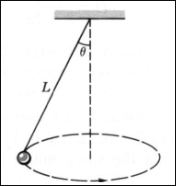
\includegraphics[scale=.5]{drawing-1.png}
\end{figure}

\subsection*{Solution}
The radius of the circle is given by
\[
	r = 1.20 \sin \theta
\]
and the centripetal acceleration is given by

\[
	a = \frac{v^2}{r}
\]
therefore, the centripetal acceleration is

\[
	a = \frac{1.28^2}{1.20 \sin 20} = \boxed{3.992\ \text{m}/\text{s}^2}
\]

\section*{Problem 7}
A stone moves in a circle of radius 60.0 cm and has a centripetal acceleration of 90 $\text{m}/\text{s}^2$. How
long does it take to make 8 revolutions?

\subsection*{Solution}
The speed of the stone is given by

\[
	v = \sqrt{ar}
\]
and the period of revolution is given by

\[
	T = \frac{2 \pi r}{v}
\]
Therefore the time it takes to make 8 revolutions is

\[
	T = 8 \frac{2 \pi 0.60}{\sqrt{90 \cdot 0.60}} = \boxed{4.104\ \text{s}}
\]


\section*{Problem 8}
Compute the acceleration for the following in terms of g's where g = 9.81 m/s2 :\\ (a) a car
moving at 100. km/h round a curve of radius 50.0 m;\\ (b) a jet flying at $1.50\times10^3$ km/h and
making a turn of radius 5.00 km;\\ (c) a stone being twirled every 0.500 s at the end of a rope of
length 1.50 m;\\ (d) a speck of dust at the rim of an LP with a radius of 6.00 in. turning at 33.1
rpm;\\ (e) a molecule in a centrifuge rotating at 30,000 rpm at a radius of 15.0 cm.

\subsection*{Solution}
\subsubsection*{Part a:}
\begin{align*}
	a = \frac{27.7778^2\ \text{m/s}}{50.0\ \text{m}} =  15.432\ \text{m}/\text{s}^2 = \boxed{1.573\ g}
\end{align*}

\subsubsection*{Part b:}
\begin{align*}
	a = \frac{416.6667^2\ \text{m/s}}{5000.0\ \text{m}} =  34.7222\ \text{m}/\text{s}^2 = \boxed{3.539\ g}
\end{align*}

\subsubsection*{Part c:}
Velocity is

\[
	v = \frac{2 \pi 1.50}{0.500} = 18.8496\ \text{m}/\text{s}
\]
Then aceleration is

\[
	a = \frac{18.8496^2}{1.50} = 236.8716\ \text{m}/\text{s}^2 = \boxed{24.146\ g}
\]

\subsubsection*{Part d:}
The speed of the speck of dust is

\[
	v = \frac{2 \pi 6.0}{33.1/60.0}\ \text{in}/\text{s}
\]
Then the acceleration is

\[
	a = \frac{\left(\frac{2 \pi 6.0}{33.1/60.0}\right)^2}{6.0} \text{in}/\text{s}^2 = 19.769\ \text{m}/\text{s}^2= \boxed{2.015\ g}
\]

\subsubsection*{Part e:}
The speed of the molecule is

\[
	v =\frac{2 \pi 15.0}{30,000/60}\ \text{cm}/\text{s}
\]
Then the acceleration is

\[
	a = \frac{\left(\frac{2 \pi 15.0}{30,000/60}\right)^2}{15.0}\ \text{cm}/\text{s}^2 = 2.369 \times 10^5 \text{m}/\text{s}^2 = 2.415 \times 10^6\ g
\]

\end{document}
